%% -*- mode: latex; mode:flyspell -*-
\documentclass[svgnames,x11names]{beamer}

\usepackage[british]{babel}

\usepackage{minted,tikz,tcolorbox,calc,siunitx}
\usetikzlibrary{chains,positioning,calc,shadows,arrows,matrix}
\usetikzlibrary{shapes.geometric,shapes.symbols}
\usetikzlibrary{circuits,circuits.logic,circuits.logic.IEC}

\usepackage{pgfplots}
\usepackage{booktabs,inconsolata}
\usepackage{bytefield}

\title{Bit Operations}
\subtitle{CM0506 -- Small Embedded Systems}
\date{Lecture 4a}
\author{Dr Alun Moon}
\institute{Department of Computer and Information Science}

\definecolor{NUblue}{RGB}{62,141,165}
\definecolor{NUbluedark}{RGB}{40,119,143}

\usetheme{CambridgeUS}

\usecolortheme{crane}
\setbeamercolor*{palette primary}{use=structure,fg=white,bg=NUblue}
\setbeamercolor*{palette quaternary}{fg=white,bg=NUbluedark}
\setbeamercolor{section in head/foot}{fg=white,bg=NUbluedark}
\setbeamercolor{subsection in head/foot}{fg=white,bg=NUblue}
\setbeamercolor{frametitle}{fg=NUbluedark!150,bg=NUblue!40}
\setbeamercolor{title in head/foot}{fg=white,bg=NUblue}
\setbeamercolor{author in head/foot}{fg=white, bg=NUbluedark}
\setbeamercolor{date in head/foot}{fg=white, bg=NUblue!60}
\setbeamercolor{title}{fg=NUbluedark!150,bg=NUblue!30}
\setbeamercolor{date}{fg=NUbluedark!150}
\setbeamercolor{block title}{fg=white,bg=NUblue}

\usepackage[T1]{fontenc}
\usepackage[utf8]{inputenc}

\begin{document}

\frame\maketitle

\begin{frame}{Boolean Algebra}{The mathematics of logic, true/false, 1/0}
\begin{description}[<+->]
\item[Values] are :\\[1ex]
\begin{tabular}{lll}\toprule
  True& 1 & High\\
  False & 0 & Low\\\bottomrule
\end{tabular}

\item[Operations] are:\\[1ex]
  \begin{tabular}{lcc}\toprule
    And & $a.b$ & $a\vee b$ \\
    Or  & $a+b$ & $a\wedge b$ \\
    Not & $\bar{a}$ & $\neg a$ \\
Exclusive Or & \multicolumn{2}{c}{$a\oplus b$}\\\bottomrule
  \end{tabular}
\end{description}
\end{frame}

\begin{frame}[fragile]{And $a \vee b$}
  \begin{block}{Truth Table}
    \begin{columns}[onlytextwidth]
      \begin{column}{.3\textwidth}
        \begin{tabular}{cc|c}
          $a$ & $b$ & $a \vee b$ \\\midrule
          0 & 0 & 0 \\
          0 & 1 & 0 \\
          1 & 0 & 0 \\
          1 & 1 & 1 \\
        \end{tabular}
      \end{column}
      \begin{column}{.5\textwidth}
        \begin{tikzpicture}[circuit logic IEC]
          \matrix[column sep=4ex] {
            \node (a) {a}; & & \\
            & \node [and gate] (g) {}; & \node (o) {$a\vee b$}; \\
            \node (b) {b}; & & \\
          };
          \draw (a.east) -- ++(right:2ex) |- (g.input 1);
          \draw (b.east) -- ++(right:2ex) |- (g.input 2);
          \draw (g.output) -- (o.west);
        \end{tikzpicture}
      \end{column}
  \end{columns}
  \end{block}

  \begin{alertblock}{Identities}
    \[ a \vee 0 = 0 \]
    \[ a \vee 1 = a \]
  \end{alertblock}
\end{frame}

\begin{frame}[fragile]{Or $a \wedge b$}
  \begin{block}{Truth Table}
    \begin{columns}[onlytextwidth]
      \begin{column}{.3\textwidth}
        \begin{tabular}{cc|c}
          $a$ & $b$ & $a \wedge b$ \\\midrule
          0 & 0 & 0 \\
          0 & 1 & 1 \\
          1 & 0 & 1 \\
          1 & 1 & 1 \\
        \end{tabular}
      \end{column}
      \begin{column}{.5\textwidth}
        \begin{tikzpicture}[circuit logic IEC]
          \matrix[column sep=4ex] {
            \node (a) {a}; & & \\
            & \node [or gate] (g) {}; & \node (o) {$a\vee b$}; \\
            \node (b) {b}; & & \\
          };
          \draw (a.east) -- ++(right:2ex) |- (g.input 1);
          \draw (b.east) -- ++(right:2ex) |- (g.input 2);
          \draw (g.output) -- (o.west);
        \end{tikzpicture}
      \end{column}
  \end{columns}
  \end{block}

  \begin{alertblock}{Identities}
    \[ a \wedge 0 = a \]
    \[ a \wedge 1 = 1 \]
  \end{alertblock}
\end{frame}

\begin{frame}[fragile]{Not $\neg a $}
  \begin{block}{Truth Table}
    \begin{columns}[onlytextwidth]
      \begin{column}{.3\textwidth}
        \begin{tabular}{c|c}
          $a$ & $\neg a$ \\\midrule
           0 & 0 \\
           1 & 1 \\
        \end{tabular}
      \end{column}
      \begin{column}{.5\textwidth}
        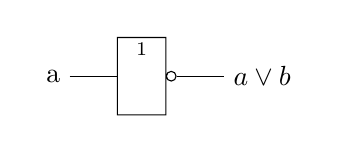
\begin{tikzpicture}[circuit logic IEC]
          \matrix[column sep=4ex] {
            \node (a) {a}; & 
             \node [not gate] (g) {}; & \node (o) {$a\vee b$}; \\
          };
          \draw (a.east) -- ++(right:2ex) |- (g.input);
          \draw (g.output) -- (o.west);
        \end{tikzpicture}
      \end{column}
  \end{columns}
  \end{block}

  \begin{alertblock}{Identities}
    \[ a \wedge 0 = a \]
    \[ a \wedge 1 = 1 \]
  \end{alertblock}
\end{frame}

\begin{frame}[fragile]{Exclusive Or $a \oplus b$}
  \begin{block}{Truth Table}
    \begin{columns}[onlytextwidth]
      \begin{column}{.3\textwidth}
        \begin{tabular}{cc|c}
          $a$ & $b$ & $a \wedge b$ \\\midrule
          0 & 0 & 0 \\
          0 & 1 & 1 \\
          1 & 0 & 1 \\
          1 & 1 & 0 \\
        \end{tabular}
      \end{column}
      \begin{column}{.5\textwidth}
        \begin{tikzpicture}[circuit logic IEC]
          \matrix[column sep=4ex] {
            \node (a) {a}; & & \\
            & \node [xor gate] (g) {}; & \node (o) {$a\vee b$}; \\
            \node (b) {b}; & & \\
          };
          \draw (a.east) -- ++(right:2ex) |- (g.input 1);
          \draw (b.east) -- ++(right:2ex) |- (g.input 2);
          \draw (g.output) -- (o.west);
        \end{tikzpicture}
      \end{column}
  \end{columns}
  \end{block}

  \begin{alertblock}{Identities}
    \[ a \oplus 0 = a \]
    \[ a \oplus 1 = \neg a \]
  \end{alertblock}
\end{frame}


\begin{frame}[fragile]{C Operators}{Bitwise logic operators}
  \begin{description}
  \item[And] ~ \makebox[34ex][r]{\mintinline{c}{a & b}} \linebreak 
    \begin{tabular}{cccccccc}
      0&0&0&1&0&1&1&0 \\
      1&0&0&1&1&0&0&1 \\\midrule
      0&0&0&1&0&0&0&0
    \end{tabular}\\[2em]

  \item[Or] ~ \makebox[34ex][r]{\mintinline{c}{a | b}} \linebreak
    \begin{tabular}{cccccccc}
      0&0&0&1&0&1&1&0 \\
      1&0&0&1&1&0&0&1 \\\midrule
      1&0&0&1&1&0&1&1
    \end{tabular}

  \end{description}
  
\end{frame}

\begin{frame}{Operating on bits}
Often we want to operate on a single bit (or group of bits) within a register.
\begin{itemize}
\item IO configuration
\item Direction bits
\item Output bits
\end{itemize}

\pause
We can use a combination of \alert{masks} and \alert{bitwise operators} to
\begin{itemize}
\item Set
\item Clear
\item Test
\end{itemize}
the state of individual bits.
\end{frame}

\begin{frame}[fragile]{Masks and notations}
Often a \alert{bitmask} is a pattern of zeros and ones marking a bit-of-interest.

\begin{example}
  For an \alert{8} bit register, we are interested in bit 5\\[1ex]
  \begin{itemize}
  \item The \emph{mask} is
\raisebox{-1ex}{
    \begin{bytefield}[endianness=big]{8}
      \bitheader{0-7}\\\bitboxes*{1}{00100000}
    \end{bytefield}}

\item in C this can be created using \alert{shift} operators
  \begin{minipage}{0.8\linewidth}
    \begin{block}{}
      \mint{c}{(1<<5)}
    \end{block}
  \end{minipage}
\item Usually given a name describing the bit it corresponds to
  \begin{minipage}{0.8\linewidth}
    \begin{block}{}
      \mint{c}{enum { led=(1<<5) };}
    \end{block}
  \end{minipage}
  \end{itemize}
\end{example}
\end{frame}

\begin{frame}[fragile]{Setting bits}
  \begin{itemize}
  \item use the \alert{or} identities $a \wedge 1 = 1$ and $a \wedge 0 = a$
  \item Or the register with the mask, writing the result back into the register
    \begin{minipage}{0.8\linewidth}
      \begin{block}{}
        \mint{c}{ dir = dir | led;}
      \end{block}
    \end{minipage}\\
  or\\
  \begin{minipage}{0.8\linewidth}
    \begin{block}{}
      \mint{c}{ dir |= led; }
    \end{block}
  \end{minipage}
  \end{itemize}

  \begin{example}
    \begin{itemize}
    \item 
    Register is
      \raisebox{-1ex}{
        \begin{bytefield}[endianness=big]{8}
          \bitboxes*{1}{11000011}
        \end{bytefield}
      }
    \item Applying the mask \texttt{led} as above
    \item  gives \raisebox{-1ex}{
        \begin{bytefield}[endianness=big]{8}
          \bitboxes*{1}{11100011}
        \end{bytefield}
      }
    \end{itemize}
  \end{example}
\end{frame}

\begin{frame}[fragile]{Clearing bits}
  \begin{itemize}
  \item use the \alert{and} identities $ a \vee 0 = 0$ and $a \vee 1 = a$
  \item Here we use \alert{and} with \alert{not}
    \begin{minipage}{0.8\linewidth}
      \begin{block}{}
        \mint{c}{ dir = dir & ~but;}
      \end{block}
    \end{minipage}\\
 or\\
 \begin{minipage}{0.8\linewidth}
   \begin{block}{}
     \mint{c}{ dir &= ~but; }
   \end{block}
 \end{minipage}
  \end{itemize}

  \begin{example}
    \begin{itemize}
    \item 
    Register is
      \raisebox{-1ex}{
        \begin{bytefield}[endianness=big]{8}
          \bitboxes*{1}{11100011}
        \end{bytefield}
      }
    \item Applying a mask defined as
      \begin{minipage}{0.8\linewidth}
        \begin{block}{}
          \mint{c}{enum { but=(1<<6) };}
        \end{block}
      \end{minipage}
    \item gives \raisebox{-1ex}{
        \begin{bytefield}[endianness=big]{8}
          \bitboxes*{1}{10100011}
        \end{bytefield}
      }
    \end{itemize}
  \end{example}
\end{frame}

\begin{frame}[fragile]{Toggling bits}
  \begin{itemize}
  \item use the \alert{exclusive or} identities $ a \oplus 1 = \neg a$ and $a \oplus 0 = a$
  \item Here we use \alert{xor}
    \begin{minipage}{0.8\linewidth}
      \begin{block}{}
        \mint{c}{ dir = dir ^ func;}
      \end{block}
    \end{minipage}\\
  or\\
  \begin{minipage}{0.8\linewidth}
    \begin{block}{}
      \mint{c}{ dir ^= func; }
    \end{block}
  \end{minipage}
  \end{itemize}

  \begin{example}
    \begin{itemize}
    \item 
    Register is
      \raisebox{-1ex}{
        \begin{bytefield}[endianness=big]{8}
          \bitboxes*{1}{10110011}
        \end{bytefield}
      }
    \item Applying a mask defined as
      \begin{minipage}{0.8\linewidth}
        \begin{block}{}
          \mint{c}{enum { func=(3<<1) };}
        \end{block}
      \end{minipage}
    \item gives \raisebox{-1ex}{
        \begin{bytefield}[endianness=big]{8}
          \bitboxes*{1}{101100101}
        \end{bytefield}
      }
    \end{itemize}
  \end{example}
\end{frame}


\begin{frame}[fragile]{Testing bits}
  \begin{itemize}
  \item use the properties of \alert{and} with the behaviour of C
  \item \alert{and} the \alert{mask} with the register
    \begin{minipage}{0.8\linewidth}
      \begin{block}{}
        \mint{c}{ pin & but; }
      \end{block}
    \end{minipage}
  \item if the result is
    \begin{itemize}
    \item 0 the bit is 0
    \item not-0 the bit is 1
    \end{itemize}

  \end{itemize}
\end{frame}

\begin{frame}[fragile]{Testing bits}
\begin{example}
    \begin{itemize}
    \item with the \texttt{pin}  
    Register as
      \raisebox{-1ex}{
        \begin{bytefield}[endianness=big]{8}
          \bitboxes*{1}{10110011}
        \end{bytefield}
      }
    \item and a mask defined as
      \begin{minipage}{0.8\linewidth}
        \begin{block}{}
          \mint{c}{enum { but=(1<<6) };}
        \end{block}
      \end{minipage}
      \begin{minipage}{0.8\linewidth}
        \begin{block}{}
          \mint{c}{pin & but}
        \end{block}
      \end{minipage}
\item      gives \raisebox{-1ex}{
        \begin{bytefield}[endianness=big]{8}
          \bitboxes*{1}{00000000}
        \end{bytefield}
      }
    \item C tests this as false
      \begin{minipage}{0.8\linewidth}
        \begin{block}{}
\begin{minted}{c}
        if( pin & but) {
          button = pressed;
        }
\end{minted}
        \end{block}
      \end{minipage}
    \end{itemize}
  \end{example}
\end{frame}

\begin{frame}[fragile]{Testing bits}
\begin{example}
    \begin{itemize}
    \item with the \texttt{pin}  
    Register as
      \raisebox{-1ex}{
        \begin{bytefield}[endianness=big]{8}
          \bitboxes*{1}{11110011}
        \end{bytefield}
      }
    \item and a mask defined as
      \begin{minipage}{0.8\linewidth}
        \begin{block}{}
          \mint{c}{enum { but=(1<<6) };}
        \end{block}
      \end{minipage}

      \begin{minipage}{0.8\linewidth}
        \begin{block}{}
          \mint{c}{pin & but}
        \end{block}
      \end{minipage}
\item
      gives \raisebox{-1ex}{
        \begin{bytefield}[endianness=big]{8}
          \bitboxes*{1}{01000000}
        \end{bytefield}
      }
    \item C tests this as true ($2^6=64$)
      \begin{minipage}{0.8\linewidth}
        \begin{block}{}
\begin{minted}{c}
        if( pin & but) {
          button = open;
        }
\end{minted}
        \end{block}
      \end{minipage}
    \end{itemize}
  \end{example}
\end{frame}



%%%% --------
\end{document}
%% Local Variables:
%% mode: reftex
%% mode: auto-fill
%% mode: flyspell
%% End:
